\documentclass[conference]{IEEEtran}
\IEEEoverridecommandlockouts
% The preceding line is only needed to identify funding in the first footnote. If that is unneeded, please comment it out.
\usepackage{cite}
\usepackage{amsmath,amssymb,amsfonts}
\usepackage{algorithmic}
\usepackage{graphicx}
\usepackage{textcomp}
\usepackage{xcolor}
\usepackage{verbatim}
\usepackage{mathtools, nccmath}
%KHOA BEGIN
\usepackage{multirow}
\usepackage{array}
%KHOA END

\ifCLASSOPTIONcompsoc
    \usepackage[caption=false, font=normalsize, labelfont=sf, textfont=sf]{subfig}
\else
\usepackage[caption=false, font=footnotesize]{subfig}

\def\BibTeX{{\rm B\kern-.05em{\sc i\kern-.025em b}\kern-.08em
    T\kern-.1667em\lower.7ex\hbox{E}\kern-.125emX}}
\begin{document}

\title{Optimal reserved resources to ensure the repetitions in Ultra-Reliable Low-Latency Communication Uplink Grant-free transmission\\
%{\footnotesize \textsuperscript{*}Note: Sub-titles are not captured in Xplore and
%should not be used}
%\thanks{Identify applicable funding agency here. If none, delete this.}
}

\author{\IEEEauthorblockN{Trung-Kien Le, Florian Kaltenberger}
\IEEEauthorblockA{\textit{EURECOM} \\
%\textit{name of organization (of Aff.)}\\
Biot, France \\
Emails: first name.last name@eurecom.fr}
\and
\IEEEauthorblockN{Umer Salim}
\IEEEauthorblockA{\textit{TCL Communication} \\
%\textit{name of organization (of Aff.)}\\
Paris, France \\
Emails: umer.salim@tcl.com}
%\and
%\IEEEauthorblockN{3\textsuperscript{rd} Given Name Surname}
%\IEEEauthorblockA{\textit{dept. name of organization (of Aff.)} \\
%\textit{name of organization (of Aff.)}\\
%City, Country \\
%email address}
%\and
%\IEEEauthorblockN{4\textsuperscript{th} Given Name Surname}
%\IEEEauthorblockA{\textit{dept. name of organization (of Aff.)} \\
%\textit{name of organization (of Aff.)}\\
%City, Country \\
%email address}
%\and
%\IEEEauthorblockN{5\textsuperscript{th} Given Name Surname}
%\IEEEauthorblockA{\textit{dept. name of organization (of Aff.)} \\
%\textit{name of organization (of Aff.)}\\
%City, Country \\
%email address}
%\and
%\IEEEauthorblockN{6\textsuperscript{th} Given Name Surname}
%\IEEEauthorblockA{\textit{dept. name of organization (of Aff.)} \\
%\textit{name of organization (of Aff.)}\\
%City, Country \\
%email address}
}

\maketitle

\begin{abstract}
To meet the strict requirements of Ultra-Reliable Low-Latency Communication in the uplink, grant-free uplink transmission has been specified, allowing the UE to transmit data in a random-access fashion without first transmitting a scheduling request and then waiting for a uplink grant from the gNB. To further increase the reliability, these grant-free uplink transmissions can be repeated without waiting for HARQ feedback from the gNB. However, these repetitions have to happen within a certain interval to avoid a confusion in HARQ IDs of different HARQ processes. When a UE starts transmitting late in the interval, it, therefore, can not exploit all the possible repetitions and thus reliability and latency decrease. In this paper, a scheme based on reserved resources is proposed to ensure the number of repetitions in a specific period. The size of each reserved resource is optimized depending on its position so as to reduce resource consumption. The scheme evaluated by theoretical analysis and numerical results shows its benefits to system performance.
\end{abstract}

\begin{IEEEkeywords}
5G, URLLC, repetitions, uplink scheduling scheme, reserved resources
\end{IEEEkeywords}

\section{Introduction} \label{I}
In 5G New Radio (NR), Ultra-Reliable Low-Latency Communication (URLLC) is one of the key features specified by The 3rd Generation Partnership (3GPP) to serve the applications such as augmented virtual reality, tactile internet and industrial automation. This new service poses a huge challenge due to a high demand of two conflicting factors: reliability and latency. The requirement for URLLC is specified in \cite{b6}: ``A general URLLC reliability requirement for one transmission of a packet is 10\textsuperscript{-5} for 32 bytes with a user plane latency of 1 ms''. Besides the baseline URLLC performance, the next release of 3GPP aims to achieve higher requirements: ``Higher reliability (up to 10\textsuperscript{-6}), higher availability, short latency in the order of 0.5 to 1 ms, depending on the use cases (factory automation, transport industry and electrical power distribution)''\cite{b8}.

\subsection{Techniques accepted in 3GPP Release 15}\label{IAA}
In Release 15, new aspects have been made and agreed by 3GPP to support URLLC. 

One of the aspects is a permission to use larger subcarrier spacings (SCS). In 5G, SCS is allowed to have a value up to 240 kHz instead of an unique value of 15 kHz as in LTE \cite{ad2}. This decision brings down transmission duration of packets from 1ms down to 62.5$\mu$s. Mini-slot based transmission further helps to reduce latency and transmission duration of packets \cite{ad3}. A user (UE) can be scheduled in a period of one or several symbols rather than a whole slot. 

The third aspect is related to the uplink (UL) transmission in grant-free (GF) region to reduce the time consumption of scheduling request (SR) and uplink grant (UL grant) \cite{ad4}. The base station (gNB) can configure a set of GF resources to one or more UEs with a periodicity defined by parameters in RRC from higher layer. When a UE is configured to transmit in GF resources, it can transmit data immediately instead of sending SR and waiting for UL Grant as grant-based (GB) transmission.

\subsection{Repetition problem in URLLC GF UL transmission}\label{IBB}
As mentioned in Section \ref{IAA}, in UL transmission, the gNB configures the UEs with high priority and strict requirements to transmit in the GF regions. In addition, it also configures the number of repetitions $K$ that these UEs need to carry out by a parameter repK from higher layer in order to guarantee transmission’s reliability. The UEs retransmit the packets automatically in the GF regions without waiting for Hybrid automatic repeat request (HARQ) feedback or UL grant from the gNB. However, the UEs are only allowed to do repetitions in one interval with a periodicity $P$ ranging from several symbols to several slots (a set of allowed periodicities $P$ is defined in \cite{ad5}) and prohibited to retransmit packet as configured by repK crossing boundary of that interval. This constraint is to help the gNB avoid a confusion in HARQ identities (IDs) of different HARQ processes. Therefore, depending on the arrival time of data in relation to the periodicity $P$, the number of repetitions might be smaller than the configured number because the UEs need to stop their transmission at the last transmission occasion in the period $P$.

\begin{figure}[htbp]
\centerline{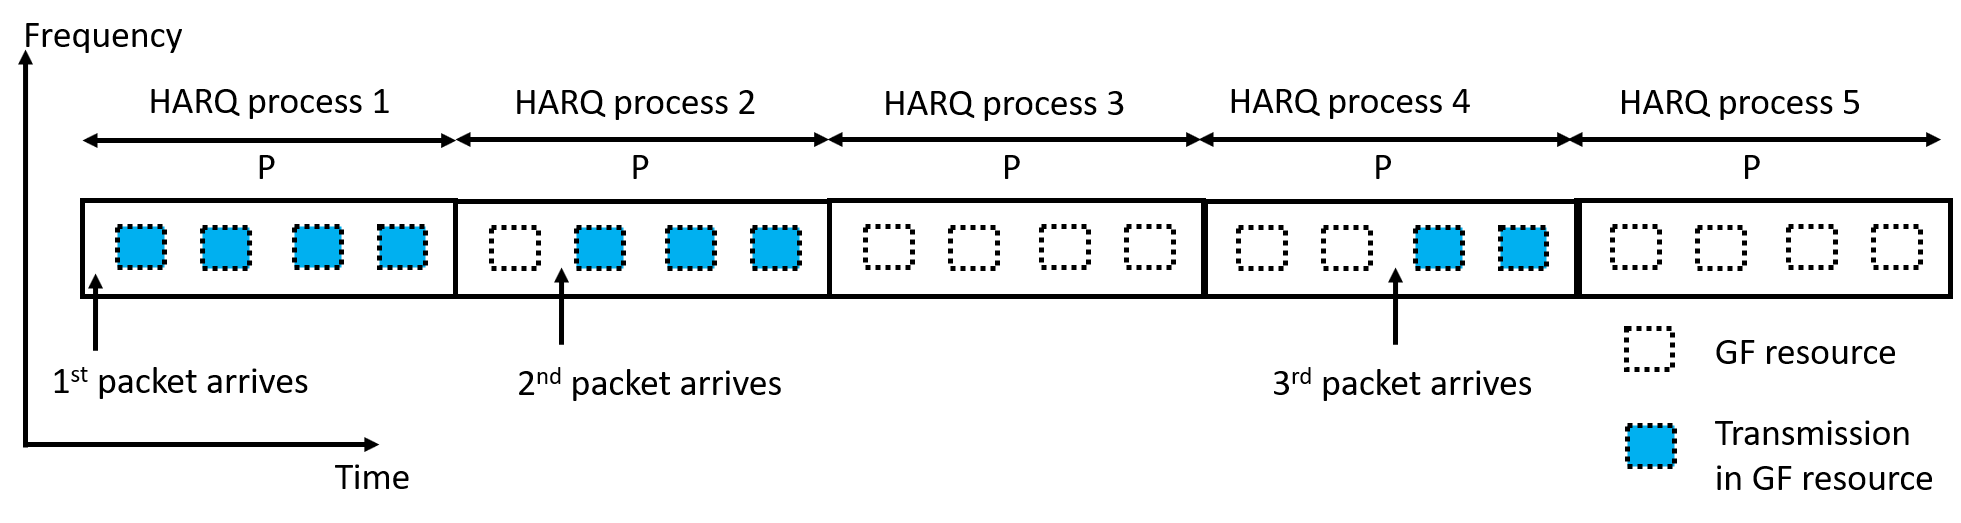
\includegraphics[scale=0.27]{fig1.png}}
\caption{Less than K repetitions in GF UL transmission.}
\label{fig1}
\end{figure}

Fig.~\ref{fig1} illustrates the situation when the number of configured repetitions is not ensured due to the constraint of boundary of period $P$. In Fig.~\ref{fig1}, an interval $P$ contains 4 GF occasions, the UE is configured to do 4 repetitions. In the first period, data comes before all the 4 GF occasions so the UE is able to do 4 repetitions for the first packet as configured. However, when data comes in the second period, there are only 3 GF occasions left in that period. This means that the UE only can carry out 3 repetitions that are less than the configured number. Similarly, in the fourth period, the UE only can transmit the packet 2 times.

It is evident that when the packet comes after the first GF occasions in a period, the UE transmits the packet with a smaller number than the number configured by repK. It degrades the reliability of UL transmission. The situation becomes more severe for the URLLC UEs with high reliability requirement. Moreover, latency of a transmission also increases because the UE needs to wait the gNB to decode the packets and transmit an UL grant to reschedule a retransmission if necessary.

\subsection{Prior art}\label{ICC}
In 3GPP Release 15, the only option for the UE is to wait until the next period to start the transmission and fulfill the configured number of repetitions. Nevertheless, this option causes big delay and prevents the UE from meeting the URLLC latency requirement, especially for low SCS. 

In \cite{b1} and \cite{b2}, repetitions are allowed to cross the boundary of a periodicity when the UE cannot make the requiring repetitions. This solution leads to a confusion of HARQ ID that makes the UE not differentiate the initial transmission and the retransmissions in order to combine and decode a specific codeblock. Besides that, a new mechanism needs to be defined to communicate explicitly HARQ ID from the UE to the gNB and results in overhead and effort in standardization.  

Multiple configurations in GF region are proposed in \cite{b3} and \cite{b4}. A UE is configured with configurations having different time offsets so it can choose the nearest configuration to start a transmission and guarantee the number of repetitions. The main concern of multiple configurations is the control overhead and delay because of signals used to configure the UE as well as resource consumption if resources in the configurations are not overlapped.

\cite{b5} and \cite{b7} propose to use shared resource for URLLC repetitions to improve resource utilization. However, they do not count a constraint that the UE cannot do repetitions crossing the border of a period. If this constraint is not solved, it might lead to a number of repetitions smaller than the configured number. In addition, shared resources are allocated periodically with the same size for all transmission occasions. These two drawbacks bring an increase of resource consumption and a drop of reliability.

In this work, an UL GF transmission scheme with reserved resources is described. Reserved resources are used and shared among the UEs when they need to transmit repetitions crossing the border of a transmission period P in order to achieve the target number of repetitions. These reserved resources have different sizes that are optimized based on the positions of their transmission occasions.  
Firstly, reserved resources and calculations to optimize their sizes are presented in Section \ref{II}. The process allowing the UEs to access to these resources is also discussed. Section \ref{III} shows numerical results obtaining from the equations derived in diverse scenarios. Finally, Section \ref{IV} provides the concluding remarks for this work.

\section{Strategy to ensure the configured number of repetitions in UL GF transmission}\label{II}

\subsection{Reserved resources}\label{IIAA}
To make the URLLC UEs achieve the strict requirements, a strategy to ensure that the UEs can transmit the number of repetitions as configured by repK from higher layer is indispensable. Reserved periodic resources are proposed to be created and assigned to multiple UEs by the gNB so that they are likely to retransmit data in case the transmissions in the reserved resources are necessary to ensure the configured number of repetitions. These reserved resources have the same periodicity as the GF resources.

\begin{figure}[htbp]
\centerline{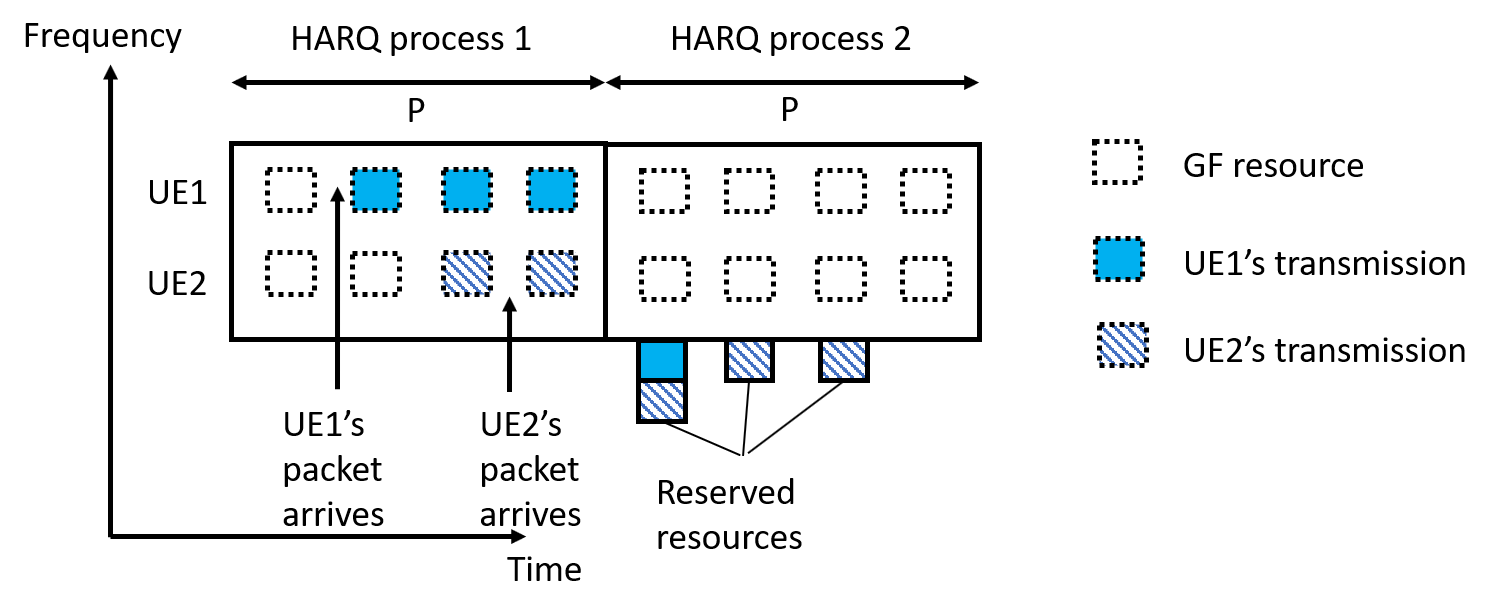
\includegraphics[scale=0.30]{fig2.png}}
\caption{Reserved resources for repetitions.}
\label{fig2}
\end{figure}

The use of reserved resources is shown in Fig.~\ref{fig2}. There are 2 UEs considered with GF resources in different bandwidth and each UE is configured with repK = 4. UE1's data comes after the first GF occasion in the first period so it only can do 3 repetitions in the period. In order to attain 4 repetitions, the UE1 retransmits data in the first reserved resource of the next period. Similarly, UE2's data arrives at the last GF occasion and only one repetition can be made. Thus, the UE2 uses the 3 reserved resources in the next period to achieve the configured number of repetitions.

In the example, 4 repetitions are configured so 3 reserved resources are needed in the next period. To increase the efficiency of resource consumption, the reserved resources are shared among the UEs. The first reserved resource in Fig.~\ref{fig2} with 2 blocks is likely to be shared with more than 2 UEs while still attain the target collision probability being approximate to the collision probability in the GF resources. Similarly, the second and third reserved resources are also shared by a group with more than 2 UEs. The equation showing the relation among the number of UEs, the size of the reserved resources and the collision probability is derived in Section \ref{IICC}.

\subsection{System model}\label{IIBB}

\begin{figure}[htbp]
\centerline{
\includegraphics[scale=0.25]{fig3.png}}
\caption{UL transmission resources' distribution.}
\label{fig3}
\end{figure}

The system in Fig.~\ref{fig3} considered to calculate collision probability in the reserved resources contains $N$ UEs. These $N$ UEs are configured by the gNB to transmit in the periodical GF resources with the number of repetitions $K$ set by parameter repK. The GF resources in one frequency band can be shared among the UEs in a group. A period $P$ corresponding to a HARQ process consists of GF transmission occasions equal to the number of repetitions $K$. The results derived below are also valid if the number of GF transmission occasions in a period are bigger than $K$. 
The reserved resources are configured periodically in each period $P$. These resources are shared among the $N$ UEs to retransmit data in case the number of repetitions that they can carry out in one period are less than the configured one. Each reserved resource has size of $M_{i}$ blocks with index $i$ indicating that the reserved resource is at the $i$th transmission occasion of a period. The size of each block in the reserved resources is the same as that of the GF resource in one transmission occasion.

The arrival of data for each UE follows a Poisson process with the average number of random access events in an interval $\lambda$ calculated from the period between the GF resources $T$ and an average packet inter-arrival time $\mu$: $\lambda$ = $T/\mu$.

\subsection{Collision probability in reserved resources}\label{IICC}
With random access, the $N$ UEs in system are allowed to use any block in the reserved resources of a specific transmission occasion if they need to do the transmissions in order to fulfill the configured number of repetitions.

The collision probability in the reserved resource at the first transmission occasion of a period (at t21 in Fig.~\ref{fig3}) is calculated as follow by considering 1 UE of interest having a transmission in the reserved resource at t21 and the rest of (N-1) UEs . 
In time $T$ between two GF resources, the probability that one UE has one or more random transmissions is \useshortskip

\begin{equation}
P_{data} = 1 - e^{-\lambda},\label{eq1}
\end{equation}

The GF resources in one bandwidth can be shared between a group of the UEs so collision probability in the GF resources between the UE of interest and other UEs of group is \useshortskip

\begin{equation}
P_{c\_GF} = 1 - e^{-\lambda(N_\mathrm{UE\_group}-1)},\label{eq2}
\end{equation}
where $N_\mathrm{UE\_group}$ is the number of the UEs that use the same frequency band of GF resources.

The reserved resource at t21 is used by a UE if its data comes after the first GF transmission occasion at t11. The probability that one UE has transmission after the first GF transmission occasion in a period $P$ is \useshortskip

\begin{equation}
P_{d} = 1 - (1-P_{data})^{K-1}.\label{eq3}
\end{equation}

There is no collision in the first reserved resource of a period $P$ at t21 if no UE rather than the UE of interest has a transmission after the first GF transmission occasion at t11. The probability that no other UE from the set of $N-1$ UEs has a transmission after the first GF occasion is calculated by \useshortskip

\begin{equation}
P_{0} = (1-P_{d})^{N-1}.\label{eq4}
\end{equation}

In case other UEs in a set of $N-1$ UEs has a transmission after the first GF occasion, the probability that $n$  UEs have such transmission is \useshortskip

\begin{equation}
P_{n} = \binom {N-1}{n}P_{d}^{n}(1-P_{d})^{N-1-n}.\label{eq5}
\end{equation}

The probability that the UE of interest and $n$ UEs do not access the same resource block in the first reserved resource at t21 is \useshortskip

\begin{equation}
P_{a0\_n} = (\frac {M_{1}-1}{M_{1}})^{n}.\label{eq6}
\end{equation}

The probability that the UE of interest does not collide with any other UE in the first reserved resource at t21 is calculated by \useshortskip

\begin{equation}
P_{sum} = \sum_{n=1}^{N-1} P_{n}P_{a0\_n}.\label{eq7}
\end{equation}

From \eqref{eq4} and \eqref{eq7}, the collision probability in the first reserved resource for the UE of interest is derived as \useshortskip

\begin{align}
P_{c1} &= 1 - P_{0} - P_{sum} \nonumber\\
 &= 1 - (\frac{M_{1}-1+e^{-\lambda(K-1)}}{M_{1}})^{N-1}.\label{eq8}
\end{align}

Based on the same calculating process, a general equation of collision probability for the reserved resource at any transmission occasion in a period can be derived as \useshortskip

\begin{equation}
P_{ci} = 1 - (\frac{M_{i}-1+e^{-\lambda(K-i)}}{M_{i}})^{N-1},\label{eq9}
\end{equation}
where
$i \in [1, K-1]$ is index indicating the position of the reserved resource based on the position of transmission occasion in a period.

\subsection{Optimization of reserved resource size}\label{IIDD}
From \eqref{eq9} with a set of parameters  $\lambda, N, K, i,$ and $P_{ci}$, the size of the reserved resources at any transmission occasion can be calculated. To guarantee the reliability of transmission in the reserved resources in comparison to that in the GF resources, the target probability $P_{ci}$ is chosen to be approximate to $P_{c\_GF}$ in \eqref{eq3}. If $P_{ci}$ is set to have the same value in all the reserved resources, the trend of reserved resources' size in terms of their positions in a period is: $M_1 > M_2 > M_3 > ... > M_{K-1}$. The size of the reserved resources to achieve a target probability decreases gradually from the first to the last reserved resource in a period. The design of the reserved resources following this decreasing trend instead of using the same size for all of the reserved resource brings an efficiency of resource consumption because the size is optimized particularly for each reserved resource.

\subsection{Group access to the reserved resources}\label{IIEE}
In group access approach, one UE is only allowed to access and uses a specific part of the reserved resource pre-configured by the gNB. One part of the reserved resource is assigned and shared among a group of the UEs. For example, the UE1-3 is only permitted to access the resource blocks as shown in Fig.~\ref{fig4}. On the other hand, other UE groups are also prohibited to access the resource blocks pre-configured to the UE1-3. 

\begin{figure}[htbp]
\centerline{
\includegraphics[scale=0.35]{fig4.png}}
\caption{Group access to the reserved resource.}
\label{fig4}
\end{figure}

For a group of the UEs accessing to a part of the reserved resources, the collision probability is calculated by \eqref{eq9} as random access approach. The size of the whole reserved resource in each transmission occasion is sum of all parts assigned to the UE groups to guarantee a target probability. 

Simulation in Section \ref{III} shows that the sizes of the reserved resources for both random access and group access approach are the same to achieve an equal target probability. However, group access approach reduces the decoding burden in the gNB. To decode a retransmitted packet, the gNB only needs to search a part of the reserved resource instead of the entire reserved resource as random access approach. Thereby, power consumption and processing time drop dramatically. 

When two or more UEs of the same group having access to a part of the reserved resources have data coming at the same time and need to use the reserved resource for repetitions, they will compete for the same part of the reserved resources at the consecutive transmission occasions as show in Fig.~\ref{fig5}. The UE 1 and 2 have 3 repetitions and data coming after the first two GF occasions so they compete two times at both the first and second reserved resources with the arrangement in the blue circle.

\begin{figure}[tbp]
\centerline{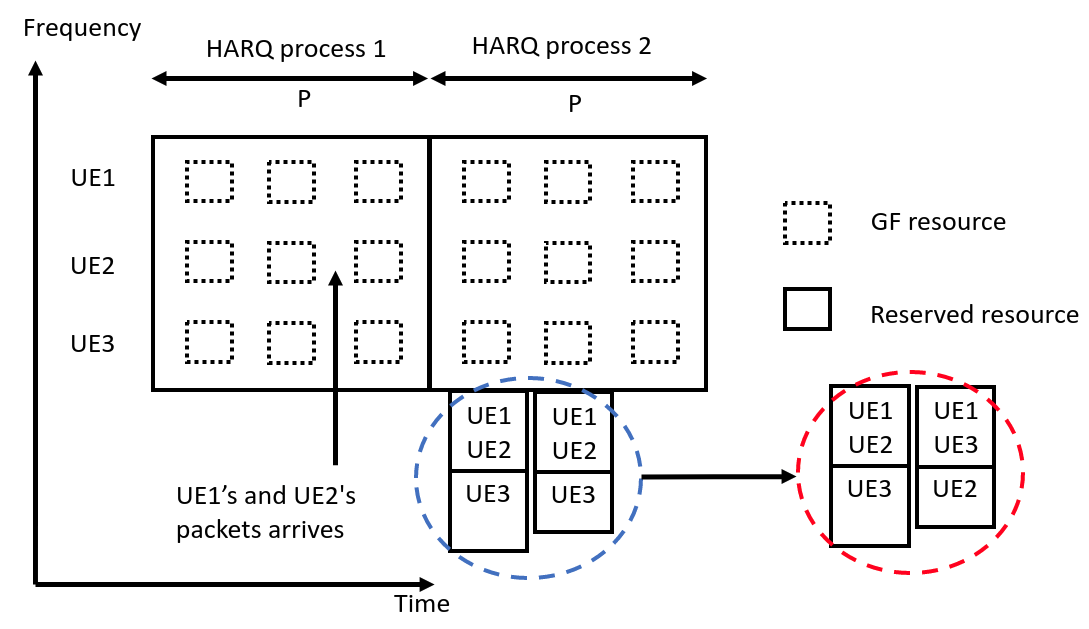
\includegraphics[scale=0.21]{fig5.png}}
\caption{Method to group the UEs in different transmission occasions.}
\label{fig5}
\end{figure}

To avoid that problem, the UEs are assigned to different groups of the reserved resources for different transmission occasions as illustrated in the red circle. The UE 1 only has the competition in both two reserved resources when both the UE 2 and 3 need to use the part of the reserved resources assigned to the UE 1 so the probability of having a competition decreases from $P_{data}$ to $P_{data}^2$ with $P_{data}$ calculated from \eqref{eq1}.



In each reserved resource, the collision probability is still the same as calculated from \eqref{eq9} but the overall reliability of a UE transmitting in the reserved resources at different transmission occasions will be improved with the hopping of the UEs to various groups in the different reserved resources.

\begin{comment}
\subsection{Explicit HARQ-ACK feedback}\label{IIFF}
In UL GF transmission, there is no HARQ feedback transmitted from the gNB to the UE to inform whether data is decoded correctly or not. The mechanism used to terminate a transmission is time-based structure. The UEs carry out the repetitions automatically as configured and data is considered to be transmitted successfully after a certain timer configured by a parameter ConfiguredGrantTimer expires. If data is not decoded, the gNB sends a UL grant to allocate resources and request the UEs to retransmit data. With this mechanism, there is a waste of time and frequency resources for the unnecessary retransmissions in case the gNB can decode correctly data before the maximum number of repetitions or the end of the timer. Moreover, if the UEs need to use the reserved resources to attain the maximum number of repetitions, the redundant data transmitted might cause a collision with data of other UEs that really need to be transmitted in the reserved resource to achieve reliability.

Therefore, when the UEs transmit less than the configured repetitions in a period and need to use the reserved resources, an explicit HARQ-ACK feedback is expected from the gNB to prevent the UEs from doing the unnecessary transmissions in the reserved resources. The presence of an explicit ACK feedback reduces resource consumption for retransmission, the sizes of the reserved resources as well as increases reliability of the transmission.
\end{comment}
\section{Numerical results and performance evaluation}\label{III}

\subsection{Random access to the reserved resources}\label{IIIAA}
From \eqref{eq9}, the number of the UEs that the system can support can be found. Besides, the number of resource blocks in each reserved resource are also calculated to sustain that system.

The simulation starts with the reserved resource in the first transmission occasion of a period. The set of parameters is $M_1=10, K=4, \lambda=1.25\times10^{-4}$.

Fig.~\ref{fig7}\subref{7a} shows collision probability in the reserved resource in the first transmission occasion in terms of the number of the UEs sharing that resource. From the graph, we see that if the target collision probability ($P_{c1}$) is 10\textsuperscript{-3}, the system can support 28 UEs in the first reserved resources.

\begin{figure}[htbp]
\centering
\subfloat[Collision probability with respect to the number of the UEs.\label{7a}]{%
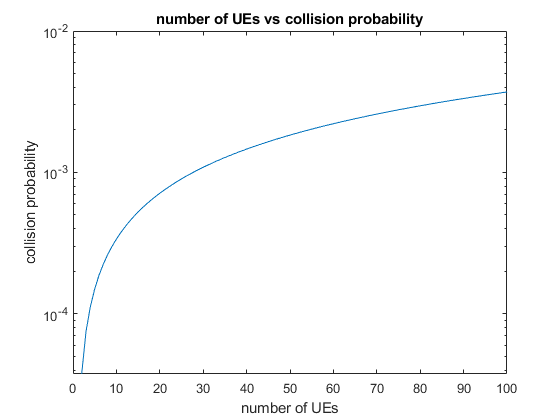
\includegraphics[scale=0.275]{fig7.png}}
\hfill
\qquad
\subfloat[Collision probability of the second reserved resource.\label{7b}]{%
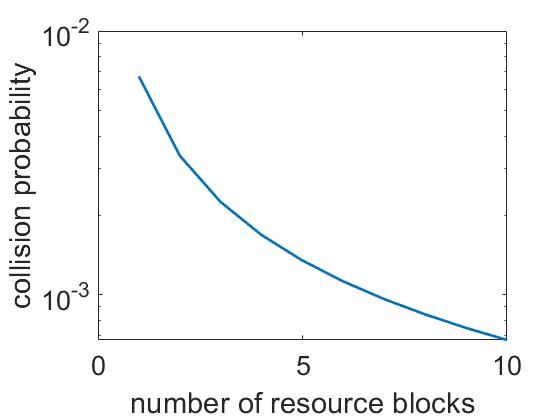
\includegraphics[scale=0.275]{fig8.png}}
\hfill
\caption{Collision probability.}
\label{fig7}
\end{figure}

\begin{comment}
\begin{figure}[htbp]
\centerline{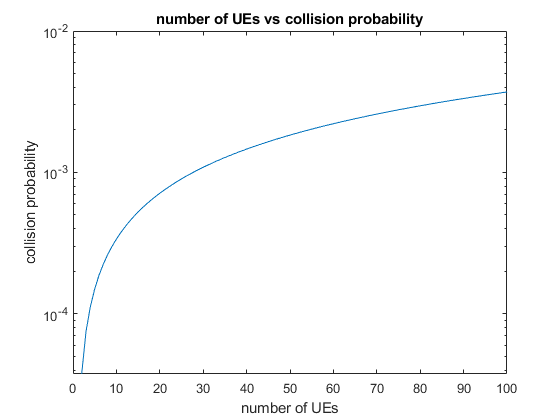
\includegraphics[scale=0.32]{fig7.png}}
\caption{Collision probability with respect to the number of the UEs.}
\label{fig7}
\end{figure}
\end{comment}

As mentioned in Section \ref{IIBB} and \ref{IICC}, the GF resources in a frequency band can be shared by a group of the UEs. 28 UEs calculated above can be divided in to 4 groups with 7 UEs in each group. The collision probability in the GF resources calculated from \eqref{eq2} is $7.5\times10^{-4}$ that is approximate to the collision probability of 10\textsuperscript{-3} in the reserved resource.

When all the parameters ($\lambda, N, K$ and $P_{ci}$) are kept the same, the sizes of the reserved resources in the second and the third transmission occasions are calculated as shown in Table~\ref{tab1}.
%KHOA BEGIN
% THem ti khoang trong' duoi table, chon medskip, bigskip hoac smallskip
%\smallskip
%\smallskip
%\bigskip
\begin{table}[htbp]
\caption{Sizes of the reserved resources with $K=4$ and random access}
\begin{center}
\begin{tabular}{|p{10em}|p{2em}|p{2em}|p{2em}|}
 \hline
 \textbf{\textit{Position of reserved resources}} & $1$ &$2$ &$3$ \\ 
 \hline
 \textbf{\textit{Number of blocks}} & $10$ &$7$ &$3$ \\

%  increase row height, number of & = number of collumn
% &&&&&\\[-1em]
 
 \hline
\end{tabular}
\label{tab1}
\end{center}
\end{table}

%\medskip
%KHOA END

The percentage of resources saved in comparison to using the same size of 10 resource blocks for all the resources in \cite{b5} and \cite{b7} is: $(1 - (10+7+3)/(10\times3))\times100\% = 33\%$.

Fig.~\ref{fig7}\subref{7b} illustrates collision probability with respect to the reserved resource's size in the second transmission occasion.

\begin{comment}
\begin{figure}[htbp]
\centerline{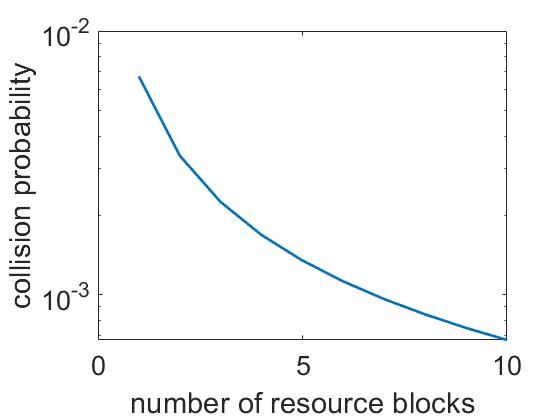
\includegraphics[scale=0.32]{fig8.png}}
\caption{Collision probability of the second reserved resource.}
\label{fig8}
\end{figure}
\end{comment}

Another scenario is considered with a bigger number of repetitions: $M_1=10, K=8, \lambda=1.25\times10^{-4}$ .

The system can support 12 UEs in the first reserved resources to achieve Pc target of 10\textsuperscript{-3}. These UEs can be divided into 2 groups with 6 UEs in one group that each group uses the GF resources in one bandwidth part. The collision probability in GF regions of a group of 6 UEs as scheduled above is: $6.25\times10^{-4}$.
With 12 UEs, the sizes of the reserved resources in the transmission occasions are shown in Table~\ref{tab2}.

\begin{table}[htbp]
\caption{Sizes of the reserved resources with $K=8$ and random access}
\begin{center}
\begin{tabular}{|p{5em}|p{2em}|p{2em}|p{2em}|p{2em}|p{2em}|p{2em}|p{2em}|}
 \hline
 \textbf{\textit{Position of reserved resources}} & $1$ &$2$ &$3$ & $4$ &$5$ &$6$ &$7$\\ 
 \hline
 \textbf{\textit{Number of blocks}} & $10$ &$8$ &$7$ & $6$ &$4$ &$3$ &$2$\\

%  increase row height, number of & = number of collumn
% &&&&&\\[-1em]
 
 \hline
\end{tabular}
\label{tab2}
\end{center}
\end{table}

The percentage of resources saved in comparison to using the same size of 10 resource blocks for all the resources in \cite{b5} and \cite{b7} is: $(1 - (10+8+7+6+4+3+2)/(10\times7)) \times100\% = 42.86\%$

As can be seen from two scenarios, the use of reserved resources with optimization from \eqref{eq9} brings an efficiency of resource utilization, especially for high configured number of repetitions. The resources needed are less than the approach of choosing blindly the same sizes for all reserved resources in different transmission occasions while still guarantees the number of repetitions with a target reliability.

Moreover, in the conventional scheme in 3GPP Release 15, the UE needs to wait until the next period if it cannot do the configured number of repetitions in the current period to fulfill the reliability requirement. Therefore, with $K=4$ and 4 transmission occasions in a period, in the worst case, the UE must wait 3 transmission occasions equal to 3 slots or 0.75ms with SCS 60kHz. This latency is close to the URLLC requirement of 1ms and causes the UEs not be able to make 4 repetitions as configured in the next period. In comparison, the proposed scheme allows the UE to start the transmission immediately and reach the configured number of repetitions in target latency of 1ms (4 repetitions consume 1ms with SCS 60kHz) as well as meet the reliability requirement.

\subsection{Group access to the reserved resources}\label{IIIBB}
Group access is simulated with the parameters as the first scenario in random access: $N = 28, K = 4, \lambda = 1.25\times10^{-4}$.

28 UEs are divided into 4 groups of 7 UEs to access the reserved resources. Each group is only allowed to access the part of the reserved resources pre-configured to them. 

To satisfy Pc=10\textsuperscript{-3}, the sizes of the reserved resources are shown in Table~\ref{tab3}.

\begin{table}[htbp]
\caption{Sizes of the reserved resources with K=4 and group access}
\begin{center}
\begin{tabular}{|p{14em}|p{2em}|p{2em}|p{2em}|}
 \hline
 \textbf{\textit{Position of reserved resources}} & $1$ &$2$ &$3$ \\ 
 \hline
 \textbf{\textit{Number of blocks per group of reserved resources}} & $2$ &$2$ &$1$ \\
 \hline
\textbf{\textit{Total number of blocks of reserved resources}} & $8$ &$8$ &$4$ \\
%  increase row height, number of & = number of collumn
% &&&&&\\[-1em]
 
 \hline
\end{tabular}
\label{tab3}
\end{center}
\end{table}

The resource consumption is equal for random access and group access to the reserved resources as shown in Table~\ref{tab1} and Table~\ref{tab3}. However, with group access, the complexity and processing time of decoding in the gNB reduce substantially because in the reserved resource at the first transmission occasion, the gNB only needs to find data of a UE in 2 reserved blocks instead of finding blindly data of a UE in 10 reserved blocks as in random access approach.

\section{Conclusion}\label{IV}

This paper presents an approach with reserved resources shared among the UEs that allows them to carry out repetitions and reach the configured number so that reliability and latency requirements can be  satisfied. Each reserved resource has an optimized size to balance reliability and  resource consumption. 

\begin{thebibliography}{00}
\bibitem{b5} R. breu, G. Berardinelli, T. Jacobsen, K. Pedersen and P. Mogensen, ``A Blind Retransmission Scheme for Ultra-Reliable and Low Latency Communications'', 2018 IEEE 87th Vehicular Technology Conference (VTC Spring), June 2018.
\bibitem{b7} Z. Zhou, R. Ratasuk, N. Mangalvedhe and A. Ghosh, ``Resource Allocation for Uplink Grant-Free Ultra-Reliable and Low Latency Communications'', 2018 IEEE 87th Vehicular Technology Conference (VTC Spring), June 2018.
\bibitem{b9} B. Singh, O. Tirkkonen, Z. Li and M. A. Uusitalo, ``Contention-Based Access for Ultra-Reliable Low Latency Uplink Transmissions'',  IEEE Wireless Communications Letters, April 2018.
\bibitem{b1} Ericsson, ``Enhancement of Configured Grant for NR URLLC'', 3GPP R1-1812162, RAN1\#95, Spokane, USA, November 12--16, 2018.
\bibitem{b2} Huawei, HiSilicon, ``Enhanced UL configured grant transmissions'', 3GPP R1-1812226, RAN1\#95, Spokane, USA, November 12--16, 2018.
\bibitem{b3} Intel Corporation, ``On enhanced Configured Grant PUSCH for eURLLC'', 3GPP R1-1812506, RAN1\#95, Spokane, USA, November 12--16, 2018.
\bibitem{b4} Sony, ``Discussion on enhanced UL grant-free transmissions'', 3GPP R1-1812746, RAN1\#95, Spokane, USA, November 12--16, 2018.
\bibitem{b6} 3GPP TR 38.913 v15.0.0, ``Study on scenarios and requirements for next generation access technologies.''
\bibitem{b8} Huawei, HiSilicon, Nokia, Nokia Shanghai Bell, ``New SID on Physical Layer Enhancements for NR URLLC''. 3GPP RP-182089, TSG-RAN\#81, Gold Coast, Australia, Sept 10--13, 2018.
\bibitem{ad2} 3GPP TS 38.211 v15.3.0, ``Physical channels and modulation.''
\bibitem{ad3} 3GPP TR 38.802 v14.2.0, ``Study on new radio access technology physical layer aspects.''
\bibitem{ad4} 3GPP TS 38.214 v15.3.0, ``Physical layer procedures for data.''
\bibitem{ad5} 3GPP TS 38.331 v15.3.0, ``Radio Resource Control (RRC) protocol specification.''

\end{thebibliography}
\vspace{12pt}


\end{document}
